%==================================================================================================
%   LUKES THESIS TEMPLATE 1.2
%   -------------------------
%   This template is based upon the offcial IMM PhD Thesis template, it is enhanced with a number
%   of new features and a number of errors have fixed. This template is intended to be complied to
%   PDF using PDFLATEX and is tested using the MiKTeX 2.9 LaTeX distribution.
%   It is based on the official DTU-IMM Thesis template by Finn Kuno Christensen in 2009.
%   Small bugfixes by Kasper Laursen in 2012.
%   -------------------------
%   Last Updated: 2012-09-19
%   Contact: lthhe@imm.dtu.dk
%==================================================================================================
%
%==================================================================================================
% DOCUMENT SETUP
%==================================================================================================
\documentclass[10pt,twoside]{book}                  %Official DTU-IMM Thesis document setup
%
\usepackage[hyphens]{url}
\usepackage{bookmark}
\usepackage{listings}
\lstset{
language=java,
extendedchars=true,
basicstyle=\footnotesize\ttfamily,
showstringspaces=false,
showspaces=false,
numbers=left,
numberstyle=\footnotesize,
numbersep=9pt,
tabsize=2,
breaklines=true,
showtabs=false,
frame=single,
extendedchars=false,
inputencoding=utf8,
captionpos=b
}

\usepackage{verbatim}





%Set to 'print' for printed version, use 'net' for online version
\def\thesisversion{print}
%
%==================================================================================================
% PACKAGES
%==================================================================================================
\usepackage{LukeThesis}                             %Import Thesis base style
%input{PhDMacros}                                   %Thesis specific macros
%
\usepackage{float}
\usepackage{rotating}
\usepackage{natbib}
%==================================================================================================
% THESIS PROPERTIES (Modifiy these fields with your details)
%==================================================================================================
\def\thesisauthor{Group: ip18groupR}         %Author
\def\thesistitle{Project: Search Engine}               %Title
\def\thesishandin{December 14, 2018}                       %Submission date (Day-Month}ng
\def\thesisdegree{Master of Science in Software Development}                              %Degree ('B.Eng', 'B.Sc.', 'M.Sc.' or 'PhD')
\def\thesisyear{2018}                               %Submission year
\def\thesisnumber{}                             %Serial number (do not include year)
\def\thesisISSN{}                          %ISSN number
\def\thesiskeywords{}  %PDF keywords
\derivethesisprops                                  %Derive dependent properties
%
%==================================================================================================
% SECTION NUMBERING SETUP
%==================================================================================================
\setcounter{tocdepth}{2}                            %2 adds sections up to subsections
\setcounter{secnumdepth}{3}                         %Subsubsections get a number when this is 3
%
%==================================================================================================
% THESIS STRUCTURE  (Modifiy to include more chapters etc)
%==================================================================================================
\begin{document}
    %------------------------
    %Pre-frontmatter material
    %------------------------
    \prefrontmatter
    %--------------------
    %Frontmatter material
    %--------------------
    %\frontmatter
    %\pagenumbering{roman}                               %Set frontmatter numbering style
    %\chapter{Summary (English)}

The goal of the thesis is to ...                                   %English summary of Thesis
    %\markboth{}{}                                       %Set headings (left)(right)
    %\input{SummaryDK}                                   %Danish summary of Thesis
    %\markboth{}{}                                       %Set headings (left)(right)
    %\chapter{Preface}

This thesis was prepared at the department of Informatics and Mathematical Modelling at the Technical University of Denmark in fulfilment of the
requirements for acquiring an M.Sc. in Informatics.

The thesis deals with ...

The thesis consists of ...
%==================================================================================================
% SIGNATURE AREA
%==================================================================================================
\vspace{20mm}
\begin{center}
    \hspace{20mm} Lyngby, \thesishandin-\thesisyear
    \vspace{5mm}
    \newline
  %Update signature image file in line below
    
\includegraphics[scale=0.5]{figures/SignatureDummy}
\end{center}
\begin{flushright}
    \thesisauthor
\end{flushright}
% % % EOF % % %                                     %Preface
    %\markboth{}{}                                       %Set headings (left)(right)
    %\input{Acknowledgements}                            %Acknowledgements
    %\markboth{}{}                                       %Set headings (left)(right)
    %------------------
    % Table of contents
    %------------------
    \newpage\mbox{}\newpage
    \chaptermark{Contents}
    \pdfbookmark{\contentsname}{toc}
    \renewcommand{\sectionmark}[1]{\markright{#1}}
    \sectionmark{Contents}
    \addtolength{\parskip}{-\baselineskip}
    \tableofcontents
    \addtolength{\parskip}{\baselineskip}
    \renewcommand{\sectionmark}[1]{\markright{\thesection\ #1}}
    %-------------
    % Main content
    %-------------
    \mainmatter
    \section{Introduction}
\label{sec:Introduction}
The goal of this project is to develop search engine as part of the Introductory Programming course at the IT University of Copenhagen. Sections 2- 4 are reporting the solutions on the mandatory tasks posted in the project description, namely Faster Queries using an Inverted Index, Refined Queries and Ranking Algorithms. Each of the mandatory tasks contain description of the\\ 


\begin{enumerate}
\item Taks, which is introduction of the task that have to be solved in the given section;
\item Basic Approach, which describes the solution;
\item Technical description, explaining the software architecture used in the solution;
\item Testing considerations, considering the corresctness of the solution;
\item  Benchmark/ Reflection, includes benchmarking results or other conclusions based on the observations or theoretical considerations;
\end{enumerate}

Besides the mandatory tasks, the challenge of the implementating OkapiBM25 algorithm for the task Ranking Algorithms have been solved as well. Several extensions also have been implemented, namely


\begin{enumerate}
    \item Changes to the client GUI
    \item Implementation of the WebCrawler
\end{enumerate}


\section{GitHub}
\label{sec:GitHub}

The source code that accompanties this report as a singel zip dile called ip18groupR.zip has been handed alongside with this report. 
The code is also available on ITU's GitHub: https://github.itu.dk/wilr/ip18groupR

\section{Statement of Contribution}
\label{sec:Statement of Contribution}
All authors contributed equally to all parts of the mandatory tasks. Ashley Rose Parsons Trew took up the challange of implementing  OkapiBM25 algorithm for the task Ranking Algorithms, Hugo Brito made the graphic design and the client GUI extension, Ieva worked with the WebCrawler extension and Jonas Hartmann Andersen enabled the team to successfully work whith this GitHub. 
    \chapter{Faster Queries using an Inverted Index}

\section{Task}
When using an search engine, the most important aspect is to be able to perform a search and get the results almost instantaneously. One way of doing this is by using an Inverted Index, which sorts the websites according to the words contained in each website. Hence when searching for a specific term, instead of going over every website, it will go over all the words instead and then provide the websites related to searched term. While building the Inverted Index can be system heavy, it is a one time operation that will allow the search engine to operate significantly faster.

\section{Basic Approach}

All the files regarding the classes mentioned on this chapter can be found on the folder src/main/java/searchengine.\\
The {\tt Index} was generalised into an interface to make it easy to test the different indices and switch between them. The following methods define the aforementioned {\tt Index} interface:
\begin{itemize}
    \item {\tt build} — Processes a list of websites into the data structure.
    \item {\tt lookup} — Given a query string, returns a list of all websites that contain such query.
    \item {\tt provideIndex} — Provides all websites in a given {\tt Index} as a collection. This specific method was added for the ranking algorithm and the testing of the index.
\end{itemize}
The inverted indices were then implemented using inheritance, since both the {\tt InvertedIndexHashMap} and {\tt InvertedIndexTreeMap} can be given exactly the same methods, being only difference their individual data structure.

\section{Technical Description}
As previously stated, a generalised {\tt Index} interface was created. Each of the classes below implements this interface, visualized in \ref{fig:Index:uml}.

\begin{figure}[H]
    \centering
    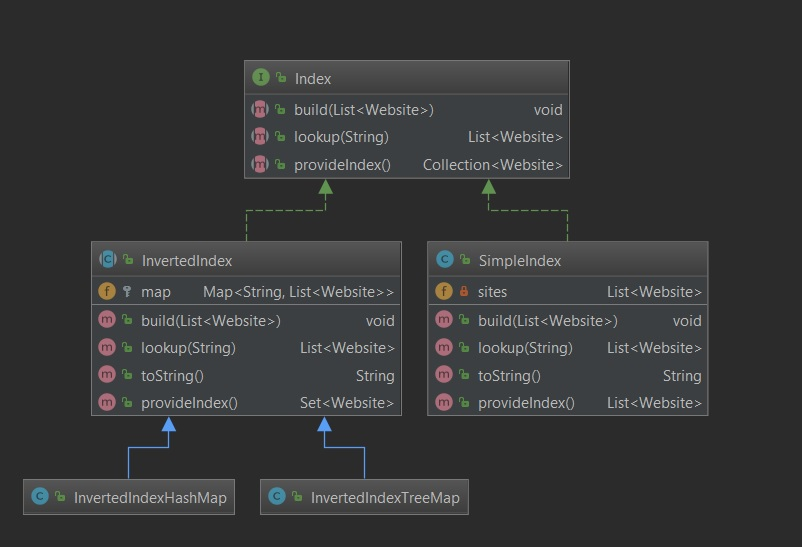
\includegraphics[width=\textwidth]{figures/Diagram_InvertedIndices}
    \caption{UML Diagram for the Software Architecture of Index data structures.}
    \label{fig:Index:uml}
\end{figure}

\subsection{{\tt SimpleIndex}}
The provided default way of indexing data was called {\tt SimpleIndex}. This solution is implemented looping through every word of every website, storing the matching website that matched the given query on an {\tt ArrayList<Website>}.\\

\subsection{{\tt InvertedIndex}}
The second (and improved) approach to index the data was to use an {\tt InvertedIndex}. As the name implies, here the relationship between a website and its words is inverted, meaning that each word knows to which sites it belongs to. In Java terms, {\tt Map}s are used where every word is a {\tt Key} with and associated {\tt Value}, which consists of an {\tt ArrayList<Website>}.\\
Since it did not make sense to create instances of {\tt InvertedIndex}, this class was made {\tt abstract} and, since it implemented methods of the {\tt Index} interface, it implements it.

\subsubsection{{\tt InvertedIndexTreeMap}}
This class {\tt extends InvertedIndex}.\\
The underlying data structure of the {\tt TreeMap} is a Red-Black tree based {\tt NavigableMap} implementation, sorted either by the natural ordering of its keys or by a {\tt Comparator}. {\tt TreeMap} provides \textit{guaranteed log(n) time} performance for the operations \textbf{containsKey}, \textbf{get}, \textbf{put}, \textbf{remove}.\cite{oracle:treemap} {\tt TreeMap} uses only the amount of memory needed to hold it's items, therefore this solution is suited when it is not known how many items have to be sorted in memory and there are memory limitations. Solutions is also suited when the order in which items have been stored is important and O(log n) search time is acceptable.\cite{baeldung:HashTreeCompared}

\subsubsection{{\tt InvertedIndexHashMap}}
This class {\tt extends InvertedIndex}.\\
The underlying data structure of the {\tt HashMap} is a hash table based implementation. This implementation provides \textit{constant-time} performance for the basic operations such as \textbf{get} and \textbf{put}.\cite{oracle:hashmap} However this is true under assumption that there are not too many collisions. This is because this {\tt Map} implementation acts as a basket hash table and when buckets get too large, they get transformed into tree nodes, similar to those of {\tt TreeMap}. \cite{baeldung:HashTreeCompared} Some of the downsides of building the HashMap are that it requires more memory than it is necessary to hold its data and when a HashMap becomes full, it gets resized and rehashed, which is costly.\cite{baeldung:HashTreeCompared}

\section{Benchmarking}
In order to choose one of the implementations, namely {\tt ArrayList}, {\tt TreeMap} or {\tt HashMap}, for the search engine, the benchmark test was performed to gain empirical data of the performance of each of the implementations. For the benchmark test, JMH (a Java harness for building, running, and analysing nano/micro/milli/macro benchmarks) was used. {OpenJDK:jmh} The benchmark test was carried out using 20 words (random nouns, verbs, adjectives and conjunctions), which were looked-up using the three different index implementations and in three different size databases: {\tt enwiki-tiny}, {\tt enwiki-small}, {\tt enwiki-medium}. JMH provides information about an average Score, measured in nanoseconds per operation, the results of which can be found in table \ref{table:result}\\
During the benchmark it was assured that the test environment is as similar as possible among the different trials, meaning that all tests were performed on the same machine and no other applications running on the background.

% Please add the following required packages to your document preamble:
% \usepackage{multirow}

\begin{table}[!h]
    \centering
    \caption{\textbf{Benchmark Scores. Each score is an average in ns/op}}
    \begin{tabular}{|l|r|r|r|l}
        \cline{1-4}
        \multicolumn{1}{|c|}{\multirow{2}{*}{\textbf{Data set}}} & \multicolumn{1}{c|}{\multirow{2}{*}{\textbf{Simple Index}}} & \multicolumn{2}{c|}{\textbf{Inverted Index}}                                  &  \\ \cline{3-4}
        \multicolumn{1}{|c|}{}                                   & \multicolumn{1}{c|}{}                                       & \multicolumn{1}{c|}{\textbf{HashMap}} & \multicolumn{1}{c|}{\textbf{TreeMap}} &  \\ \cline{1-4}
        enwiki-tiny                                              & 18 944,884                                                  & 1 052,067                             & 1 591,311                             &  \\ \cline{1-4}
        enwiki-small                                             & 8 819 338,592                                               & 1 883,776                             & 3 622,582                             &  \\ \cline{1-4}
        enwiki-medium                                            & 233 498 546,571                                             & 27 451,020                            & 30 176,993                            &  \\ \cline{1-4}
    \end{tabular}
    \label{table:result}
\end{table}

% Jonas' table, just in case.
% \begin{table}[!htbp]
%     \caption{\textbf{Benchmark Scores. Each score is an average in ns/op}}
%     \begin{tabular}{|p{75pt}|p{75pt}|p{75pt}|p{75pt}|}
%         \hline
%         \textbf{Data set} & \textbf{Simple Index} & \textbf{IE: HashMap} & \textbf{IE: TreeMap} \\ \hline
%         enwiki-tiny & 18 944,884 & 1 052,067 & 1 591,311 \\ \hline
%         enwiki-small & 8 819 338,592 & 1 883,776 & 3 622,582 \\ \hline
%         enwiki-medium & 233 498 546,571 & 27 451,020 & 30 176,993 \\ \hline
%     \end{tabular}
%     \label{table:result}
% \end{table}

The benchmark results shows that the {\tt SimpleIndex} is significantly slower than both of the {\tt InvertedIndex} implementations: 233 498 546,571 ns/op versus 27 451,020 ns/op for the {\tt InvertedIndexHashMap} and 30 176,993 ns/op for the {\tt InvertedIndexTreeMap} using the {\tt enwiki-medium} dataset.
In order to describe the results, let the number of websites be $m$ and words be $n$.
The difference in performance can be explained as follows:\\
When the {\tt SimpleIndex} is looking up the search word, it looks though all the sites, which takes \textit{O(m)} time, and for each site it looks through all the words which takes \textit{O(n)} time, therefore total search time is \textit{O($m\cdot n$)}. The two other methods provide faster performance time. InvertedIndexTreeMap provides a \textit{guaranteed} performance of \textit{O(log(n))}. InvertedIndexTreeMap provides best-case performance of constant time \textit{O(1)} and the worst-case performance of \textit{O(log(n))} time (since Java 8). Worst-case performance occurs when the hash function is not implemented correctly and values are distributed poorly in buckets, leading to high hash collision.

%$2 \cdot log(n) + occ$\
There are several considerations when choosing the implementation for storing the data for the Search Engine.

HashMap seams to be better fit than a TreeMap for Search Engine solution, because in this case the order of data is not important whereas the performance looking up the websites corresponding the search word is. The HashMap can be expected to perform in constant time which is better than TreeMap's \textit{log(n)} time, and only in the HashMap's worst-case performance is it \textit{log(n)} time. The given data sets are fixed, therefore the costly resizing and rehashing is not going to occur implementing Hashmap. HashMap performed the best on all of the given different size datasets in benchmark test. This is the reasoning for choosing HashMap implementation over the TreeMap implementation for this Search Engine project.

\section{Testing Considerations}
After the above changes were implemented, development tests were written in order determine the viability of the code and whether the changes satisfied the requirements of the task. To that end, JUnit tests were devised for each class that was updated.

\subsection{Index tests}
The correctness of the {\tt build} and {\tt lookUp} method were verified using unit tests (JUnit 5), which can be found in the {\tt IndexTest} file.
When setting up the test, a small {\tt List<Website>} was created which made it easier to predict the expected results of the methods. Each test
checks all of the indices using the white-box coverage considerations. The {\tt SimpleIndex} were more used as a reference to the others, and the
tests as it should be able to pass all test, due its simple nature.

The {\tt build} method was verified by creating a {\tt String} of what was expected the index should contain and then calling the {\tt toString} on
the index.

The {\tt lookUp} method was tested by providing it with words and then checking the size of the list returned against the expected size of that list.

Lastly, a test of checking whether the websites contained in the Index is the same as the websites read by the {\tt FileHelper} class was done.
This was performed on the tiny, small and medium files and was meant to see whether the behaviour of the index would stay the same when the
database size changed.

%How to reference surce\footnotemark.
%\footnotetext{Oracle \url{https://docs.oracle.com/javase/8/docs/api/java/util/HashMap.html}}

%How to reference surce\footnotemark.
%\footnotetext{Oracle \url{https://docs.oracle.com/javase/8/docs/api/java/util/TreeMap.html}}

% report ends before this line
    \chapter{Refined Queries}

%• Task: A short review on the task that we had to solve.
%• Basic Approach: A basic description on how we solved the task.
%• Technical description: Description of software architecture used in the solution.
%• Testing considerations: Description of considerations for testing the correctness
%of our solution.
%• Benchmarking/Reection: Benchmarking results for experiments that allowed us
%choose the best data structure for the search engine.

%Checklist for Mandatory Tasks
%Use the following checklist to make sure your project fulfills all mandatory tasks.
% Tasks 1–3 have correspondent Java code that solve them, in particular,
% you have implemented the inverted indexes, and benchmarked them,
% your searchengine understands complex queries,
% your searchengine is able to rank results to a query, using dierent scores.
% each class and each method is documented using Javadoc
% each class is accompanied with a unit test, in which you test the public methods
%exposed by the class (no tests need to be provided for main and “getter” methods)

\section{Task} % A short review on the task that we had to solve.
This task enables complex query handling. This is a basic feature that is expected from a search engine: to be able to understand queries that consist of more than just one word (intersected search). Additionally, the task required the search engine to be able to handle aggregated results from different (possibly) multi-word queries when the {\tt OR} keyword is present (unioned search).

\section{Basic Approach} % A basic description on how we solved the task.
All the logic necessary to handle the queries was implemented in the class {\tt QueryHandler}.
When considering what needs to be accomplished as well as what the user can input in the search field, the present task is accomplished by following these steps:
\begin{enumerate}
    \item Sanitise the query: this comprises of checking if the query is meaningful and fulfils basic criteria in morphological terms, and to enforce it in the cases it does not.
    \item Separate the query into sub-queries whenever the {\tt OR} keyword is present.
    \item For each of the sub-queries, find websites that contain all the words in that sub-query.
    \item Aggregate all the results of the multiple sub-queries on a list.
\end{enumerate}
In order to achieve encapsulation and responsibility-driven design, the following methods were implemented in the above-mentioned class:
\begin{itemize}
    \item {\tt getMatchingWebsites}: Core method of the class. It is responsible for:
    \begin{itemize}
        \item Receiving the input and passing it to the {\tt cleanQuery} helper method.
        \item Receiving the input from the {\tt cleanQuery} method in a meaningful and orderly fashion, passing it then, element by element, to the {\tt intersectedSearch} method.
        \item Receiving every result of the {\tt intersectedSearch} method and store it, so that when every element of the list is processed, it returns the matching websites.
    \end{itemize}
    \item {\tt cleanQuery}: Auxiliary private method to make sure that the input is free from unaccounted or irrelevant input.
    \item {\tt intersectedSearch}: Auxiliary private method that returns websites that match simultaneously all the words in the input {\tt String} parameter.
\end{itemize}

\section{Technical description} % Description of software architecture used in the solution.
\subsection{Field}
The {\tt QueryHandler} class takes an {\tt Index} object and a {\tt Score} object as the initialising parameters and assigns them to private fields. The {\tt Index} can be any of the indices described in the previous chapter as all extend the same {\tt Interface}. The same can be said for the {\tt Score} interface, and the details of this can be found in the next chapter. %This was achieved with the following piece of code:
%\begin{lstlisting}[language=Java]
%public class QueryHandler {
%private Index idx = null;
%public QueryHandler(Index idx) {
%this.idx = idx;
%}
%\end{lstlisting}
\subsection{{\tt getMatchingWebsites} core method}
As soon as this class is instantiated, its intended use expects the {\tt getMatchingWebsites} method to be called. This method takes in a {\tt String} as parameter, which consists of the search terms and returns a {\tt List<Website>}, which consists of the matching results. %The signature is as follows:
%\begin{lstlisting}[language=Java]
%public List<Website> getMatchingWebsites(String line) {
%\end{lstlisting}
As the description in the Basic Approach states, this method uses two auxiliary methods to process the data as necessary. The first data processing happens when the parameter is passed to {\tt cleanQuery} method, which then returns a list of Strings that can be used to proceed with the search. %The code used to achieve this is the following:
%\begin{lstlisting}[language=Java]
%List<String> query = cleanQuery(line);
%\end{lstlisting}
\subsection{{\tt cleanQuery} auxiliary method}
This method enforces consistency in the input to be later on used to search for results.
The first steps of the process consist of:
\begin{itemize}
    \item Replacing all the punctuation characters by spaces
    \item Replacing every one or more space characters by a single space character
\end{itemize}
The above mentioned steps are achieved by making use of the {\tt String} method {\tt replaceAll}.
%\begin{lstlisting}[language=Java]
%private List<String> cleanQuery (String input) {
%input = input.replaceAll("\\p{Punct}", " ").replaceAll("\\s+", " ");
%\end{lstlisting}
After this, the {\tt OR} keyword is used as criteria for splitting the input {\tt String} using the {\tt split} method, which is then used to create a {\tt List<String> searches}. The idea is that every element of the list will consist of an intersected search, and the search results of each element will then be aggregated to achieve the final result.
The {\tt split} method gives {\tt String []} as a result, but is then parsed as an {\tt ArrayList<String>} as this is more maleable, and through the {\tt java.util} methods allows for the consistency in the {\tt List<String> searches} to be enforced (such as trimming all the searches in case they start or end with empty spaces, deleting all empty entries in the {\tt List<String>}, and making everything lower case due to the way the website content is stored in the index). This was elegantly achieved by using lambdas.
\subsection{Intermediate steps in the {\tt getMatchingWebsites} method}
The refined search query, now stored in a {\tt List<String>}, is iterated through and each element passed as a parameter to the auxiliary method {\tt intersectedSearch}, the results of which are stored in a {\tt Set<Website> results}. The root of the reason for the choice of such data structure is the fact that it does not allow duplicates (as opposed to a {\tt List}, which expedites the process. Since we intend to iterate through a set of data, it seemed appropriate to implement a {\tt for} loop.
\subsection{{\tt intersectedSearch} auxiliary method}
Given a certain {\tt String} parameter, this auxiliary private method returns a {\tt Set<Website>} where each {\tt Website} matches simultaneously all the words in such parameter. The idea is that:
\begin{itemize}
\item The {\tt String} parameter is split by space characters using the {\tt split} method.
\item The resulting {\tt String[]} is converted to an {\tt ArrayList<String>}.
\item The {\tt lookup} method, using field {\tt Index idx}, is called on the first element in the {\tt ArrayList<String>}.
\item The result of this is stored in a {\tt HashSet<Website>}.
\end{itemize}
Should there be more than one {\tt String} in the {\tt ArrayList<String>} i.e. more than one word in the parameter {\tt String} to intersect the first set of results with, these results will be used to compare with the results of the remaining {\tt String} in the {\tt ArrayList<String>}. In order to accomplish such task, the results of every other given word were successively compared with the results from the first element of the list. The refining criteria was to keep only the websites that were present on both lists.
To this end, the {\tt Set} method {\tt retainAll} was utilised.
\subsection{Final steps in the {\tt getMatchingWebsites} method}
All the results from each of the different intersected searches performed by the {\tt getMatchingWebsites} method are added to a {\tt HashSet<Website>} (again, to avoid any duplication of websites), which is then passed to the {\tt rankWebsites} method and returned as a {\tt List<Website>}. The details of the {\tt rankWebsites} method will be discussed in more depth in the next chapter.

\section{Testing considerations} % Description of considerations for testing the correctness of our solution.
Upon testing for correctness, we split the test cases in two main groups: one that tests basic functionality, and a second one that tests for bad user behaviour.
\begin{itemize}
    \item Testing for the basic functionality:
        \begin{itemize}
            \item One word
            \item One or more words separated by spaces;
            \item Two words with the ``{\tt OR}'' keyword in between;
            \item Groups of words separated by the ``{\tt OR}'' and by spaces;
        \end{itemize}
    \item Testing for bad user behaviour, where the query:
    \begin{itemize}
        \item Is empty;
        \item Starts with white space followed by the ``{\tt OR}'' keyword;
        \item Repeats the words separated by the ``{\tt OR}'' keyword;
        \item Consists of solely the ``{\tt OR}'' keyword;
        \item Starts with the ``{\tt OR}'' keyword followed groups of words separated by spaces;
        \item Starts with white space followed by the ``{\tt OR}'' keyword followed groups of words separated by the ``{\tt OR}'' and by spaces and ends with ``{\tt OR}'' ;
        \item Consists of only white space;
        \item Starts with punctuation and white space and is followed by a group of words separated by spaces;
        \item Consists of several ``{\tt OR}'' keywords separated by spaces, followed by a group of words separated by spaces and ends with several ``{\tt OR}'' keywords separated by spaces;
        \item Consists of several words separated by the ``{\tt OR}'' keyword where there is more that one ``{\tt OR}'' occurrence between words;
        \item Contains only upper case characters;
        \item Contains no spaces but a word surrounded by several ``{\tt OR}'' keywords;
        \item Contains an upper case word next to an ``{\tt OR}'' keyword with no spaces in between, followed by another ``{\tt OR}'' keyword and a word.
        \item Lastly, we considered the worst case scenario where a query contained many of the above-mentioned cases and also for when there was punctuation between words.
    \end{itemize}
\end{itemize}

\section{Reflection} % Benchmarking results for experiments that allowed us choose the best data structure for the search engine.
Sets used to avoid duplication of results, regexs used to parse the input string quickly, arraylists over arrays for flexibility,



    \chapter{Chapter 4: Ranking Algorithms}

\section{Task}
Typically, results returned from search engines are ranked in some way so as to return the more relevant search results first.
The general idea behind this is that for a given website, a score is calculated for each word to indicate the importance of that word on the site.
Then, for intersected searches (that is, searches where all words are required to be present on the webpage for it to be a match) the score is a summation of the scores for each individual word in the search,
and for unioned searches (that is, searches where as long as either part of the union is present on the website it is a match), the score is taken as the maximum of the score for each part of the union search.
For this task, the following ranking algorithms were introduced:

\begin{itemize}

\item Term frequency

\item Term frequency - inverse document frequency

\item Okapi BM25

which are different implementations of the same aforementioned general idea: assigning a score to a search term based on some metric of relevance.

\end{itemize}

\section{Basic Approach}
Research was conducted into the implementations of each of the ranking algorithms.

\begin{itemize}

\item Term frequency
The term frequency (TF) is simply this: given a word and a document (which in this case, is a webpage), how many times does a word appears on the website.
However there are various permutations on this basic formula.
The TF formula settled on in the end was

\begin{equation*}
    term frequency = \frac{number of times the word appears on the website}{number of words on the website}
\end{equation*}

to normalise the score a bit, as a word appearing 10 times on a website 50 words long has a different significance to a word appearing 10 times on a website 500 words long.

\item Term frequency - inverse document frequency
Before the term frequency - inverse document frequency (TFIDF) algorithm can be discussed, the idea behind 'inverse document frequency' must be explained.
The idea behind the inverse document frequency is that while the number of times a word appears on a webpage is a good indication of how important that
word is to that webpage, there are many common words such as 'the', 'and', 'this' etc that will inevitably appear multiple times on a website and will
therefore skew the score of any kind of score based on term frequency.
The inverse document frequency formula is designed to take this into account and is calculated as follows

\begin{equation*}
    inverse document frequency = log_{10}(\frac{number of websites in the search engine index}{number of websites containing the word})
\end{equation*}

Taking the log of this ratio means that the more times a word appears on a website in the database, the closer the IDF gets to 0, and a word that appears on every website
in the database is awarded an IDF value of 0.
That is, common words that are likely to appears on multiple (if not all) websites will have no impact on the ranking score
\\
With that in mind, the meaning behind the TFIDF ranking algorithm becomes clear.
The TFIDF score is calculated as follows:

\begin{equation*}
    TFIDF = TF * IDF
\end{equation*}

The TF score judges the relevance of the word to the website, and the IDF is a weighting to adjust for common words.
Very common words are awarded a TFIDF score of 0 and therefore give no impact in intersected searches.

\item Okapi BM25
The Okapi BM25 algorithm is a more sophisticated type of TFIDF ranking algorithm.
It's a summation over all words that make up the search term, making use of the TF calculation as well as the IDF calculation, with optimisation variables too.
The version of the formula used in this project is:

\begin{equation*}
    okapi BM 25 score = \sum_{i=1}^n IDF(w_i) \cdot \frac{TF(w_i)\cdot (k_1 + 1)}{TF(w_i) + k_1\cdot(1 - b + b\cdot \frac{number of words on the website}{average number of words on a webpage})}
\end{equation*}

with the optimisation variables set as $k_1 = 1.2$ and $b = 0.75$ since no advanced optimisation was considered.
\end{itemize}

It was also decided that the various permutations of Score classes created would be solely responsible for the calculations.
Any required logic was to be handled by the QueryHelper class.

\section{Technical Description}
As per the task description, a generalised {\tt Score} interface was created with only one method: {\tt getScore} which performs the score calculation for the given word with the given website, taking the following parameters:

\begin{itemize}
    \item @param word a word from the search query
    \item @param site the website being scored against the search string
    \item @param index the index of websites
\end{itemize}

and each of the below classes implement this interface.

\begin{figure}[t]
    \centering
    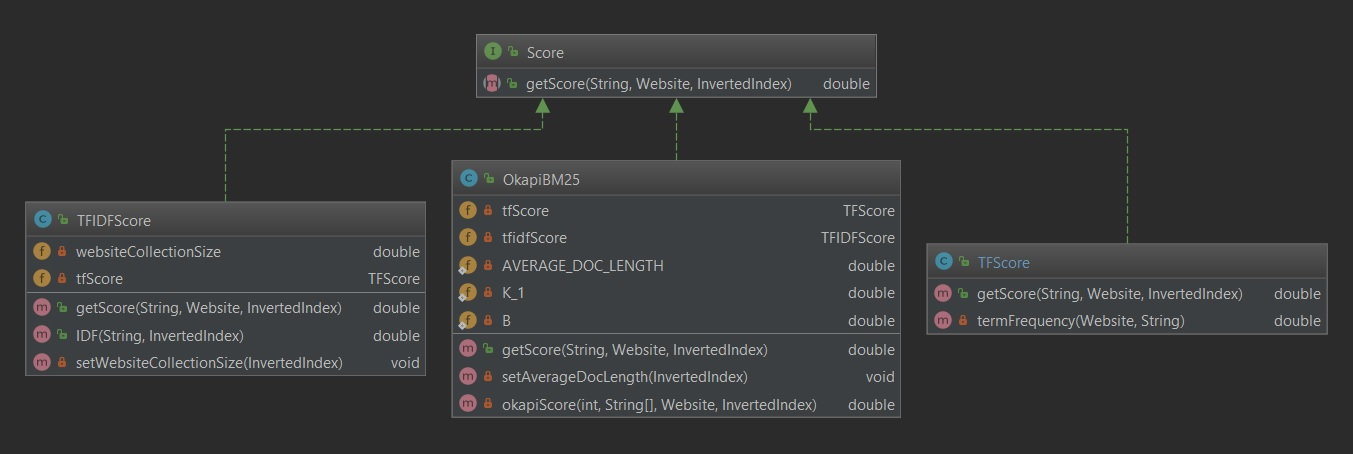
\includegraphics[width=\textwidth]{figures/diagram-score}
    \caption{UML Diagram for the Software Architecture of Score data structures.}
    \label{fig:score:uml}
\end{figure}

\subsection{IFScore class}
The {\tt TFScore} class was the simplest of the three classes to implement, as shown in Figure \ref{fig:score:uml}.
Due to the version of the term frequency formula used in this project, there is a helper method to supplement the required {\tt getScore} method, leaving the {\tt getScore} method to only handle the division.
Due to the changes made to the {\tt FileHelper} class - namely, that no website that lacks a title or words can be created - it's not possible
for there to be a divide by zero error, so no steps were made in this method to account for it.

\subsection{TFIDFScore class}
As the TFIDF makes use of the TF calculation, the {\tt TFIDFScore} class was given a field of type {\tt TFScore} with which to call methods on as needed, rather than creating a new object each time it was required.
Again, helper methods were added to deal with the different aspects of the calculation i.e. the IDF and the number of websites in the search engine index.
The number of websites in the index was built from the index {\tt Map<String, Website>} as below,

\begin{lstlisting}[language=Java]
    private void setWebsiteCollectionSize(InvertedIndex index) {
        Set<Website> siteCollection = new HashSet<>();
        Set<String> words = index.getIndexMap().keySet();
            for(String word : words) {
                List<Website> sites = index.getIndexMap().get(word);
                siteCollection.addAll(sites);
            }
        this.websiteCollectionSize = siteCollection.size();
    }
\end{lstlisting}

making use of the fact that a HashSet allows no duplicates in order to calculate the number of distinct websites in the index.
Again, the {\tt getScore method} only handles the multiplication

\subsection{OkapiBM25 class}
Again, as the Okapi BM25 algorithm makes use of both the TF calculation and the TFIDF calculation, these objects were stored as fields in the {\tt OkapiBM25Score} class as before.
The optimisation constants and the average document length set as static fields.
Two helper methods were added: {\tt setAverageDocLength} and {\tt okapiScore}. {\tt setAverageDocLength} calculates the mean number of words per website based on the websites in the index, and {\tt okapiScore} is a recursive method to perform the summation of all the individual scores of all the words in the search query to return to the {\tt getScore} method.

\begin{lstlisting}[language=Java]
    private double okapiScore(int count, String[] words, Website site, InvertedIndex index) {
        int docLength = site.getWords().size();
        if(count != 0) {
            double IDF = this.tfidfScore.IDF(words[count], index);
            double termFrequency = this.tfScore.getScore(words[count], site, index);
            double score = IDF*((termFrequency*(K_1 + 1))/(termFrequency + K_1*(1 - B + B*(docLength/AVERAGE_DOC_LENGTH))));
            return score + okapiScore(count-1, words, site, index);
        } else {
            double IDF = this.tfidfScore.IDF(words[0], index);
            double termFrequency = this.tfScore.getScore(words[0], site, index);
            return IDF*((termFrequency*(K_1 + 1))/(termFrequency + K_1*(1 - B + B*(docLength/AVERAGE_DOC_LENGTH))));
        }
    }
\end{lstlisting}

\section{Testing considerations}
The correctness of the score calculations were verified using unit tests, which can be found in the ScoreTest.java file.
The set up comprised of building a small index of websites, which allowed for the score values of various words on various
websites to be calculated manually and compared to the results of the {\tt getScore} method.
Each test covered one class, and the individual tests were determined using the standard white-box coverage considerations.
For the tests on the {\tt TFIDFScore} class, a comparison was also included to confirm that a word occurring once on more than one site will have a lower score than a word occurring once on just one site.
For the tests on the {\tt OkapiBM25Score} class, single word and multi word query tests were constructed.

\section{Reflection}

    \chapter{Extensions}


\section{Okapi BM25}

\subsection{Okapi BM25} (Basic Approach)
The Okapi BM25 algorithm is a more sophisticated type of TFIDF ranking algorithm.
It's a summation over all words that make up the search term, making use of the TF calculation as well as the IDF calculation along with variables that can be used for optimisation.
The version of the formula used in this project is:

\begin{align}
    OBM25 = \sum_{i=1}^n IDF(w_i) \cdot \frac{TF(w_i)\cdot (k_1 + 1)}{TF(w_i) + k_1\cdot(1 - b + b\cdot \frac{W}{\bar{W}})}
\label{eq:OBM25}
\end{align}

with the optimisation variables set as $k_1 = 1.2$ and $b = 0.75$ since no advanced optimisation was considered and

\begin{itemize}
    \item $OMB25$ is the Okapi BM 25 score
    \item A search term $w$ consists of individual words $w_1, w_2, ..., w_n$
    \item $IDF(w_i)$ is the inverse document frequency score applied to the word $w_i$
    \item $TF(w_i)$ is the term frequency score applied to the word $w_i$
    \item $W$ is the number of words on the webpage
    \item $\bar{W}$ is the average number of words on a webpage
\end{itemize}

\subsection{OkapiBM25Score class} (Technical Description)
As the Okapi BM25 algorithm makes use of both the TF calculation and the TFIDF calculation, these objects were stored as fields in the {\tt OkapiBM25Score} class in a similar manner to what was done for the {\tt TFIDFScore} class.
The optimisation constants and the average document length were set as static fields.
Two helper methods were added: {\tt setAverageDocLength} and {\tt okapiScore}. {\tt setAverageDocLength} calculates the mean number of words per website based on the websites in the index, and {\tt okapiScore} is a recursive method to perform the summation of all the individual scores of all the words in the search query to return to the {\tt getScore} method.

\begin{lstlisting}[language=Java]
    private double okapiScore(int count, String[] words, Website site, InvertedIndex index) {
    int docLength = site.getWords().size();
    if(count != 0) {
        double IDF = this.tfidfScore.IDF(words[count], index);
        double termFrequency = this.tfScore.getScore(words[count], site, index);
        double score = IDF*((termFrequency*(K_1 + 1))/(termFrequency + K_1*(1 - B + B*(docLength/AVERAGE_DOC_LENGTH))));
        return score + okapiScore(count-1, words, site, index);
    } else {
        double IDF = this.tfidfScore.IDF(words[0], index);
        double termFrequency = this.tfScore.getScore(words[0], site, index);
        return IDF*((termFrequency*(K_1 + 1))/(termFrequency + K_1*(1 - B + B*(docLength/AVERAGE_DOC_LENGTH))));
        }
    }
\end{lstlisting}

\subsection{OkapiBM25Score class} (Testing Considerations)
The mathematical correctness of the OBM25 score calculations were verified using unit tests, which can be found in the ScoreTest.java file alongside the unit tests for the other {\tt Score} classes.
The set up was the same as previously mentioned in the Ranking Algorithm's chapter.
Positive tests for single word and multi word query tests were constructed in the following manner:

\begin{itemize}
    \item the word doesn't occur on the specified website
    \item the word doesn't occur in the website index at all
    \item the word occurs once on the specified website
    \item the word occurs once on the specified website and at least one other website
    \item the word occurs more than once on the specified website
    \item multi-word query: words don't occur on the specified website
    \item multi-word query: words occur once on the specified website
    \item multi-word query: words occur more than once on the specified website
    \item multi-word query: words occur once on the specified website and at least one other website
    \item comparison of the above score values
\end{itemize}

Negative testing consideration were harder to formulate.
The most obvious to test would be dividing by 0, however as seen in equation \ref{eq:OBM25}, it's not actually possible for the denominator to be 0 due to the optimisation variables: either $TF(w_i)$ or $\frac{W}{\bar{W}}$ has to be negative, which is not possible.
To that end, no negative tests were considered for the {\tt OkapiBM25} class.

\section{Improve the Client GUI} % Change the client code such that the result of searches are displayed in a nicer way.

We were given the possibility to improve the front-end of the search challenge as an added task. The client side of our product consists of a set of files that dictate, among other things, the aspect of the page, implements the pieces and bits of code that will ultimately allows the user communicate with the server and perform the searches; and arranges the results of the queries in a more user-friendly fashion.\newline
The files containing the code that concerns the front-end of the search engine can be found in the folder static. Here follows each of the files' description:
\begin{itemize}
    \item index.html — This is the first file the browser reads upon accessing the root of a website hosted in any given domain. Hence it holds what other files to read also (such as the styling sheet), provides written unformatted text which will be displayed on the browser, which may also includes links to other webpages.
    \item style.css — It is possible to style a given webpage from a given html file, but it is best practice to do in on a separate file (such as the present one). Should one build a website with several pages (which for each a separate html file is necessary), styling can become cumbersome and even result in styling inconsistencies. So this file provides a styling guide that can be used for several different pages providing consistency among all of them, and for this is only necessary to add the line of code that points to such file in the html.
    \item code.js — It holds the javascript code that allows for changes in the html (or even style), which will result in changes on what the user sees. Our javascript code was responsible for receiving the search term(s), sending them to the server, receiving the results of the given search, and translating them into html.
    \item Image files in static/img/ — Some images needed to provide the website with the desired aspect.
\end{itemize}
The basic implementation of the client GUI allowed the very basic functionality of performing a search. So the accomplished tasks in this regard will be described in the following subsections.

\subsection{Adding content to be displayed by the html}
A wireframe of a preliminary graphic design of the website can be found in the appendix. Several aspects of the GUI were changed to improve the user's experience. We included a footer with links to ITU's website, the course page, as well as our LinkedIn profiles. Overall names of the classes and id's to be used in the styling sheet were also changed to achieve the intended design. Code was also added to include background images.
Additionally, it seemed intuitive to allow the enter key to trigger a search, so such feature was implemented by including a small script in the html file.

\subsection{Styling}
All the aspect of the website was described in the style.css file. In here, virtually everything was changed, namely:
\begin{itemize}
    \item Centering the content of the webpace;
    \item The aspect of every given class, id, link, as well as behaviour of certain elements when, for example, the user hovers the mouse over that specific element;
    \item Providing responsiveness no the website (adjusting the aspect of the content depending on the size of the viewport;
    \item Behaviour of the background images, where they would display as crossfaded slide show;
    \item Behaviour of the searchbar, where it would change its size by clicking on it.
\end{itemize}

\subsection{Adding functionality through javascript}
Changes in the javascript code, which can be found in the static/code.js, where made in order to allow for:
\begin{itemize}
    \item Provide a different answer depending on the given different queries. The cases we accounted for were the following:
    \begin{itemize}
        \item No query was provided;
        \item The query did not provide any result;
        \item The query in a number of results different than $0$.
    \end{itemize}
    \item Besides the title and the URL, the results are also accompanied by a certain number word from the given website.
    \item Clicking on a result will open it on a new tab (instead of the current tab).
\end{itemize}
    \chapter{Chapter 6 Conclusion}


\section{Section 6}
Text \\





    \appendix
    \chapter{Test Figure reference}
\label{appendix:figure}
This is a test of the appendix and how to reference to something in it. 
Below is shown an image which is used for test\footnotemark{testimage}. 
\footnotetext{this is just for testing...\url{www.test.dk}} 
\begin{figure}[h]
  \centering
 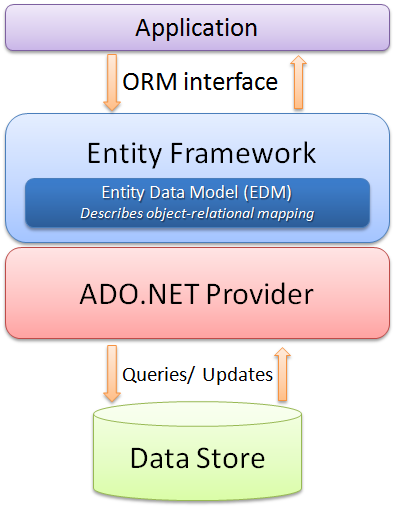
\includegraphics[scale=0.5]{figures/Entity-Framework}
  \caption{Microsoft Entity Framework}
  \label{fig:entityframework}
\end{figure}


    \chapter{Tables}
\label{app:table}

\begin{table}[H]
    \caption{Coverage table of the parseFile(String filename) method}
    \begin{tabular}{|l|p{100pt}|l|}
        \hline
        \textbf{Choice} & \textbf{Input property} & \textbf{Input data set} \\ \hline
        1 catch & incorrect file name & A \\ \hline
        1 try & file name & B \\ \hline
        2 while: zero times & empty file & B1 \\ \hline
        2 while: once & file has one line & B2 \\ \hline
        2 while: more than once & file has two lines & B3 \\ \hline
        2 while: more than once & file has at least three lines & B4 \\ \hline
        3 true & the line contains a web url & B3, B4 \\ \hline
        3 false & the line does not contain a web url & B1, B2 \\ \hline
        4 true & either the listOfWords field or the title field is null & B3, B4 \\ \hline
        4 false & both the listOfWords and the title fields are not null & B4 \\ \hline
        5 true & the url field is not null & B4 \\ \hline
        5 false & the url field is null & B3, B4 \\ \hline
        6 true & the line contains a website title & B3, B4 \\ \hline
        6 false & the line doesn't contain a website title & B2 \\ \hline
        7 true & listOfWords is null & B2, B4 \\ \hline
        7 false & listOfWords is not null & B4 \\ \hline
    \end{tabular}
    \label{tab:Coverage}
\end{table}

\begin{table}[H]
    \caption{Expectancy table of the JUnit tests}
    \begin{tabular}{|l|p{85pt}|p{100pt}|p{100pt}|}
        \hline
        \textbf{Input data set} & \textbf{Input data} & \textbf{Expected output} & \textbf{Actual output} \\ \hline
        A & "wrongfilename.txt" & Exception & FileNotFoundException \\ \hline
        B1 & "data/test-file1.txt" & returns an ArrayList<website>, size() == 0 & returns an ArrayList<website>, size() == 0 \\ \hline
        B2 & "data/test-file2.txt" & returns an ArrayList<website>, size() == 0 & returns an ArrayList<website>, size() == 0 \\ \hline
        B3 & "data/test-file3.txt" & returns an ArrayList<website>, size() == 0 & returns an ArrayList<website>, size() == 1 \\ \hline
        B4 & "data/test-file-errors.txt" & returns an ArrayList<website>, size() == 2 & returns an ArrayList<website>, size() == 2 \\ \hline
        B4 & "data/test-file4.txt" & returns an ArrayList<website>, size() == 2 & returns an ArrayList<website>, size() == 2 \\ \hline
    \end{tabular}
    \label{tab:Expectancy}
\end{table}

\begin{table}[H]
    \caption{Data Set}
    \begin{tabular}{|l|l|l|l|}
        \hline
        \begin{minipage}[c]{0.12\columnwidth}
            \textbf{data/test\\-file2.txt} \\
        \end{minipage} &
        \begin{minipage}[c]{0.24\columnwidth}
            \textbf{data/test-file3.txt} \\
        \end{minipage} &
        \begin{minipage}[c]{0.32\columnwidth}
            \textbf{data/test-file4.txt} \\
        \end{minipage} &
        \begin{minipage}[c]{0.35\columnwidth}
            \textbf{data/test-file-errors.txt} \\
        \end{minipage} \tabularnewline \hline

        \begin{minipage}[t]{0.12\columnwidth}%
            word3 %
        \end{minipage} &
        \begin{minipage}[t]{0.24\columnwidth}%
            http://example.com \\
            Title1%
        \end{minipage} &
        \begin{minipage}[t]{0.32\columnwidth}%
            *PAGE:http://page1.com \\
            Title1 \\
            word1 \\
            word2 \\
            *PAGE:http://page2.com \\
            Title2 \\
            word1 \\
            word3 %
        \end{minipage} &
        \begin{minipage}[t]{0.35\columnwidth}%
            word1 \\
            word2 \\
            *PAGE:http://page1.com \\
            Title1 \\
            word1 \\
            word2 \\
            *PAGE:http://wrong1.com \\
            Title1 \\
            *PAGE:http://wrong2.com \\
            *PAGE:http://wrong3.com \\
            Titleword1 Titleword2 \\
            *PAGE:http://page2.com \\
            Title2 \\
            word1 \\
            word3 \\%
        \end{minipage} \tabularnewline \hline
    \end{tabular}
    \label{tab:DataFiles}
\end{table}
    %-----------
    % Backmatter used for Bibliography
    %-----------
    \backmatter
    \chaptermark{Bibliography}
    \renewcommand{\sectionmark}[1]{\markright{#1}}
    \sectionmark{Bibliography}
    \addcontentsline{toc}{chapter}{Bibliography}        %Force addition of Bibliography to TOC
    \bibliographystyle{apalike}                           %Use alpha codes for references
    \bibliography{reference}                           %Bibliography file called
\end{document}
% % % EOF % % %